\documentclass[11pt,a4paper]{article}

%\usepackage{style2017}
\usepackage{hyperref}

\usepackage[T1]{fontenc} 
\usepackage[utf8]{inputenc}
\usepackage[francais]{babel}
\usepackage{url}
\usepackage{etex}
\usepackage{enumitem}
\usepackage{multicol}
\usepackage{bbm}
\usepackage{amsmath,amsthm,amssymb}
\usepackage[official]{eurosym}
%\usepackage{pifont}
\usepackage[left=1cm, right=1cm, top=1.5cm, bottom=1.5cm]{geometry}
\usepackage{exercise}
\usepackage{graphics}
\usepackage{array,multirow,makecell}
\usepackage{verbatim}
\usepackage[dvipsnames,table]{pstricks}
\usepackage{pstricks-add,pst-plot,pst-text,pst-tree,pst-eps,pst-fill,pst-node,pst-math,pst-blur,pst-func}
\usepackage{pgf,tikz}
\usepackage{tipfr}
\usepackage{thmbox}
\usepackage{calc}
\usepackage{ifthen}
\usepackage{pdfpages}
\usepackage{colortbl}
%\usepackage{sagetex}
\usetikzlibrary{arrows,patterns}
\input tabvar
\usepackage{tkz-tab}
\usepackage{listings}
\usepackage[np]{numprint}
%\usepackage{tabularx}
\usepackage{fancybox,fancyhdr}
\usepackage{thmtools}
\usepackage{bclogo}
\usepackage{lastpage}

%------------------------------------- 
%        		Abréviations personnelles
%-------------------------------------
\newcommand{\Cc}{\textbf{Conclusion : }}
\newcommand{\DNS}{\textbf{Devoir Non Surveillé}}
\newcommand{\DS}{\textbf{Devoir Surveillé}}
\newcommand\fpsd{une fonction polynôme du second degré~}
\newcommand{\N}{\mathbb{N} } % Raccourci pour l'ensemble des entiers naturels
\newcommand{\R}{\mathbb{R}} % Raccourci pour l'ensemble des réels
\newcommand{\Z}{\mathbb{Z}} % Raccourci pour l'ensemble des entiers relatifs
%\newcommand{\N}{\mathbb{N}} % Raccourci pour l'ensemble des réels

%----------------------------------------------------------------------------------------------- 
% 							Commandes mathématiques
%-----------------------------------------------------------------------------------------------
\renewcommand{\vec}[1]{\overrightarrow{#1}}	% Raccourci pour vecteurs
\newcommand{\inv}[1]{\dfrac{1}{#1}} % Raccourci pour l'inverse des réels
\newcommand{\e}{\text{e}}
\newcommand*{\E}{\ensuremath{\mathrm{e}}}
\newcommand{\lnx}{\ln(x)}

%----------------------------------------------------------------------------------------------- 
% 							Commandes Tableaux
%-----------------------------------------------------------------------------------------------
\setcellgapes{3pt}
\makegapedcells
\newcolumntype{R}[1]{>{\raggedleft\arraybackslash }b{#1}}
\newcolumntype{L}[1]{>{\raggedright\arraybackslash }b{#1}}
\newcolumntype{C}[1]{>{\centering\arraybackslash }b{#1}}

%----------------------------------------------------------------------------------------------- 
% 							Commandes Listes
%-----------------------------------------------------------------------------------------------
% Redéfinition du premier niveau
\renewcommand{\theenumi}{\arabic{enumi}}
\renewcommand{\labelenumi}{\textbf{\theenumi)}}
% Redéfinition du deuxième niveau
\renewcommand{\theenumii}{\alph{enumii}}
\renewcommand{\labelenumii}{\textbf{\theenumii)}}

%-----------------------------------------------------------------------------------------------
%							 		Environnement - Macros
%-----------------------------------------------------------------------------------------------
\setlength{\columnsep}{20pt}
\setlength{\columnseprule}{0.5pt}
\renewcommand{\thesection}{\arabic{section}}
%\renewcommand{\thesection}{\arabic{section}}
%La numérotation des section repart à 0 lorsque l'on change de partie
%\makeatletter\@addtoreset{section}{chapter}\makeatother
\makeatletter\@addtoreset{subsection}{section}\makeatother
%\renewcommand{\thechapter}{\arabic{chapter}}
%\renewcommand{\thesection}{\arabic{section}}
\renewcommand{\thesubsection}{\arabic{subsection}}
%Modifier la section dans son positionnement, sa forme, couleur,...
%\makeatletter
%\renewcommand\section{\@startsection {section}{1}{\z@}%
%                                   {-1.5ex \@plus -0.5ex \@minus -.2ex}%
 %                                  {1.8ex \@plus .2ex}%
  %                                 {\raggedleft\normalfont\color{gray}\large\bfseries}}
%\makeatother
\newenvironment{maliste}%
{ \begin{list}%
	{$\bullet$}%
	{\setlength{\labelwidth}{30pt}%
	 \setlength{\leftmargin}{35pt}%
	 \setlength{\itemsep}{\parsep}}}%
{ \end{list} }

\newenvironment{NSI}[2]
{
	\noindent
	\setlength{\fboxsep}{0cm}\setlength{\fboxrule}{0pt}\framebox[19cm]{
		\setlength{\fboxsep}{0.25cm}\setlength{\fboxrule}{1pt}
		\Huge{\textbf{#1 :}}
		\hspace{0.5cm}{\huge{#2}}\hfill
	}
	{\newline \rule[0cm]{\linewidth}{0.05em}}
}

\hypersetup{
    colorlinks =false,
    linkcolor=blue,
   linkbordercolor = 1 0 0
}
\newcounter{numexo}
\setcellgapes{1pt}
\setlength{\parskip}{8pt}

\begin{document}



\begin{NSI}
{TP}{Listes chainées en POO}
\end{NSI}

La liste chainée est composée de maillons. Chaque maillon de la liste contient une valeur et pointe sur le maillon suivant.
La liste chainée pointe sur le premier maillon de la chaine de maillons.

\section{Le maillon}

On donne l'implémentation du maillon en programmation orientée objet.

\begin{center}
\includegraphics[scale=0.8]{../img/tp_poo_1.png}
\end{center}

La classe \textsf{Maillon} définit 2 attributs et 2 méthodes:

\begin{itemize}

\item Les attributs \textsf{valeur} et \textsf{suivant} sont initialisés à la construction ou à \textsf{None} en l'absence de valeur.

\item Les méthodes pour construire l'objet et pour l'afficher.

\end{itemize}


\begin{enumerate}
\item Les maillons ci-dessous sont reliés entre eux. Ils forment une chaine.

\begin{center}
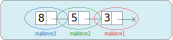
\includegraphics[scale=0.8]{../img/maillon_chaine.png}
\end{center}

\begin{enumerate}
\setlength{\itemsep}{6pt}
\item Construire un maillon \textsf{m1} qui contient la valeur 3.
\item Construire le maillon \textsf{m2} qui contient la valeur 5 et qui pointe sur le maillon \textsf{m1}.
\item Construire le maillon \textsf{m3} qui contient la valeur 8 et pointe sur le maillon \textsf{m2}.
\end{enumerate}

\item Créer un nouveau maillon \textsf{m} contenant la valeur 1. Nous allons relier ce maillon à la chaine de maillons précédente.

\begin{enumerate}
\item Le maillon \textsf{m} est placé au début de la chaine.

\begin{center}
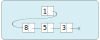
\includegraphics[scale=0.8]{../img/maillon_chaine_1.png}
\end{center}

Écrire les instructions pour réaliser cette opération et afficher la chaine.


\item Le maillon \textsf{m} est placé à la fin de la chaine.

\begin{center}
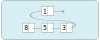
\includegraphics[scale=0.8]{../img/maillon_chaine_2.png}
\end{center}

Écrire les instructions pour réaliser cette opération et afficher la chaine.
\end{enumerate}


\item Le maillon \textsf{m} est placé dans la chaine entre la première et la deuxième valeur.

\begin{center}
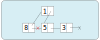
\includegraphics[scale=0.8]{../img/maillon_chaine_3.png}
\end{center}
\begin{itemize}
\item Le maillon \textsf{m} pointe sur le second maillon de la chaine
\item Le premier maillon \textsf{m3} pointe sur le maillon \textsf{m} et plus sur le maillon \textsf{m2}.
%\item On supprime la liaison entre le premier et le deuxième maillon
\end{itemize}
\begin{enumerate}
\item Écrire les instructions pour réaliser cette opération et afficher la chaine.
\item Recommencer en plaçant le maillon \textsf{m} entre le deuxième et le troisième maillon de la chaine.
\end{enumerate}

\end{enumerate}


\section{La liste chainée}

Dans la partie précédente, nous avons vu qu'il est possible de lier des maillons sous forme de chaine. 

On va créer un nouvel objet \textsf{Liste} qui a un attribut unique \textsf{maillon}. Cet attribut a pour valeur \textsf{None} si la liste est vide et un maillon si elle n'est pas vide.

La liste contient plusieurs méthodes répondant à l'interface de liste chainée.

\begin{itemize}
\item Le constructeur qui crée une liste vide.
\item La méthode \textsf{est\_vide} qui renvoie un booléen pour savoir si la liste est vide.
\item La méthode \textsf{tete} qui renvoie la tête de la liste soit la première valeur.
\item La méthode \textsf{queue} qui renvoie la queue de la liste, c'est à dire la liste sans la tête.
\item La méthode \textsf{inserer} qui prend en paramètre un élément à insérer dans la liste et l'ajoute en tête de la liste.
\end{itemize}\medskip

On reprend le fichier contenant la classe \textsf{Maillon} et on crée la classe \textsf{Liste} juste en dessous.


\begin{enumerate}
\setlength{\itemsep}{6pt}
\item Créer le constructeur de la classe \textsf{Liste} permettant de créer une liste chainée vide. 

\item Ajouter la méthode \textsf{est\_vide} qui renvoie un booléen. Une liste est vide si l'attribut \textsf{maillon} vaut \textsf{None}.

\item Ajouter la méthode \textsf{tete} qui renvoie la tête de la liste, c'est à dire la première valeur de la liste. 

\item Ajouter la méthode \textbf{queue} qui renvoie une liste constituée des éléments de la liste chainée sans sa tête. Il est donc nécessaire de créer une nouvelle liste chainée \textsf{queue} et lui attribuer le bon maillon.

\item La méthode \textbf{inserer} prend en paramètre un élément et l'insère dans la liste. Pour y parvenir, il faut créer un maillon et l'insérer en tête de la liste.

On donne le code à compléter:

\begin{center}
\includegraphics[scale=0.8]{../img/poo_liste_inserer.png}
\end{center}


\end{enumerate}

\section{Application}


\begin{enumerate}
\setlength{\itemsep}{6pt}
\item Écrire la fonction \textsf{creer\_liste()} sans paramètre qui renvoie une liste chainée vide.

\item Créer une liste vide nommée \textsf{maliste}. Vérifier que \textsf{maliste} est vide avec la bonne méthode.

\item Insérer dans la liste chainée \textsf{maliste} les voyelles \textsf{a, e, i, o, u} de notre alphabet. Afficher la liste.

\item Écrire la fonction \textsf{parcourir} qui prend en paramètre une liste chainée. Cette fonction affiche un à un les éléments de la liste chainée et ne renvoie rien.

On suivra l'algorithme ci-dessous:
\begin{itemize}
\item Il faut, dans la fonction, définir une variable locale \textsf{maillon} qui prend la valeur du premier maillon de la liste chainée.
\item Tant que la variable locale \textsf{maillon} n'est pas vide, on affiche la valeur et on passe au maillon suivant.
\end{itemize}


\item La fonction \textbf{longueur\_liste} prend en paramètre la liste et renvoie le nombre d'éléments qu'elle contient soit sa longueur. 
L'algorithme suivant peut vous guider dans son écriture:

\begin{center}
\begin{tabular}{|L{10cm}|}\hline
on crée la variable longueur à 0\\
tant que le suivant de liste n'est pas vide: \\
\hspace{1cm} la longueur augmente de 1\\
\hspace{1cm} on passe au suivant\\
on renvoie la longueur\\\hline
\end{tabular}
\end{center}

Écrire le code de la fonction en python.

\item La fonction \textsf{get\_item} prend en paramètre une liste chainée et un nombre entier \textsf{i}. Cette fonction renvoie la valeur de la liste dont l'index (position) est \textsf{i}. Par exemple, si \textsf{i=0}, on renvoie la première valeur.

Quelques remarques:
\begin{itemize}
\item On s'assure que l'argument \textsf{i} a des valeurs valides.
\item Comme pour la fonction parcourir, il faut une variable locale \textsf{maillon} qui parcourt la liste.
\end{itemize}

\item Écrire la fonction \textsf{renverse} qui renverse la liste chainée. La première valeur devient la dernière, etc. Elle prend en argument une liste chainée et renvoie une liste chainée avec les éléments en ordre inverse.


\item La fonction \textsf{ajouter\_fin} prend en paramètre une liste chainée et un élément à insérer. La fonction renvoie la liste chainée avec l'élément ajouté en fin de liste.

On suivra l'algorithme ci-dessous:
\begin{itemize}
\item Il faut parcourir la liste chainée jusqu'au dernier maillon de la chaine.
\item On fait pointer ce dernier maillon sur un nouveau maillon qui contient l'élément passé en argument.
\end{itemize}


%\item La fonction \textbf{supprime\_tete} prend en paramètre la liste. Pour supprimer la tete, il suffit :
%\begin{itemize}
%\item de vérifier si la liste est non vide. Si oui, alors la  queue de liste devient la liste.
%\item on renvoie la liste
%\end{itemize}

\item Si la liste chainée est longue, l'insertion en fin de liste nécessite de la parcourir entièrement pour insérer un nouveau maillon. Ceci n'est donc pas très optimal.

Une solution consiste à ajouter un attribut \textsf{last} à la classe \textsf{Liste} qui contient le dernier maillon de la liste chainée. Ainsi, quand on ajoute une valeur en fin de liste, il suffit de faire pointer le maillon \textsf{last} sur le maillon à insérer et d'actualiser l'attribut \textsf{last}.

Apporter les modifications nécessaires à la classe \textsf{Liste} et récrire la fonction \textsf{ajouter\_fin} en utilisant l'attribut \textsf{last}.

\end{enumerate}
\end{document}
